\chapter{多重度、熵與受限平衡}

\lectureoverview{一旦機率分布中的各個狀態具有能量，這個分布便成為熱力學對象。我們先把熵增加與平衡化連結起來，並利用\(dE=T\,dS\)推導熱流的方向。接著，我們以大量複本取代單一系統，計算每組佔據數所對應的排列數，並證明這個多重度的對數等於熵乘以\(N\)。因此，平衡問題就是在約束條件下求熵的最大值；拉格朗日乘數則提供求解所需的方法。}

\section{三個基本量}

令\(i\)標記系統可用的離散狀態。目前採用離散狀態很方便，因為我們可以直接計數，而不必引入相空間測度。若狀態\(i\)的機率為\(P_i\)，則\begin{equation}
 \sum_i P_i=1.
 \label{eq:sm3-normalization}
\end{equation}若該狀態的能量為\(E_i\)，平均能量為\begin{equation}
 \overline E=\sum_iP_iE_i.
 \label{eq:sm3-mean-energy}
\end{equation}\emph{平均}一詞很重要。系統在任何單一微觀態中都不必具有\(\overline E\)這個值；它是各種可能值依機率加權所得的平均。

\begin{classroomqa}\classquestion{這裡的機率與統計之間，是否有值得區分之處？}\lecturerresponse{機率為可能結果提供模型；統計通常則從觀測資料出發，探問能據此推論什麼。本計算使用機率分布，不過同樣的平均值也自然會出現在統計資料中。課堂上的這段非正式問答對兩個詞的用法較為寬鬆，因為這項區別不影響接下來的物理內容。\lecturetimestamp{00:01:39--00:02:21}}\end{classroomqa}

分布的熵為\begin{equation}
 S[P]=-\sum_iP_i\log P_i.
 \label{eq:sm3-entropy}
\end{equation}此式非負。每個非零機率都滿足\(0<P_i\leq1\)，因此\(\log P_i\leq0\)；當\(P_i\to0\)時，則採用通常的極限值\(P_i\log P_i\to0\)。

\begin{figure}[t]\centering
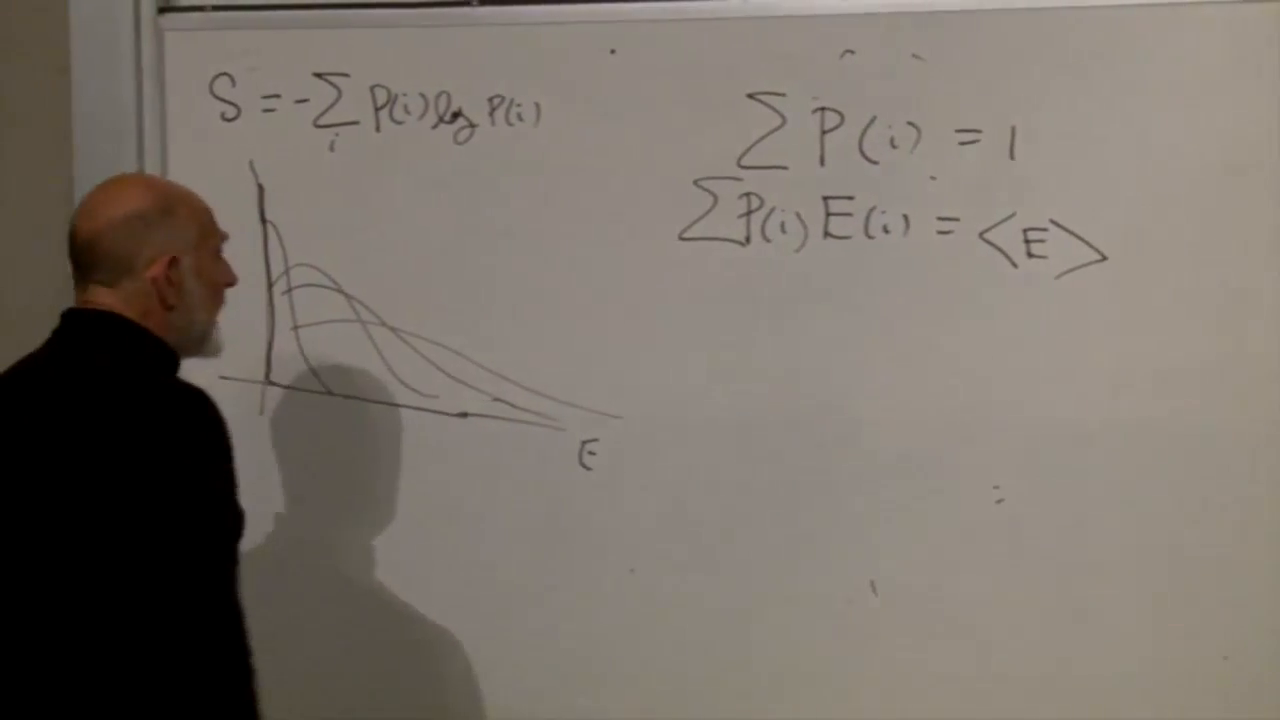
\includegraphics[width=0.88\textwidth]{lecture_03_figure_02.png}\caption{開場板書將熵、歸一化與平均能量的公式，以及一系列定性描繪的平衡分布，一併列出。}\lectureframe{00:06:44}\end{figure}

\section{作為一族分布的平衡}

上一講留下了一族由單一參數標記的平衡分布。雖然可以用溫度標記這一族分布，但目前用平均能量\(\overline E\)來標記更為方便。在可能的最低能量下，分布集中於基態：\[
 P_i=\delta_{i0}.
\]此時我們對系統所處的狀態毫無不確定性，且\(S=0\)。平衡分布涵蓋的能階愈多，其平均能量與熵也都愈大。

這個敘述只適用於熱平衡分布這一族，並非適用於任意構造的分布族。任意一族分布可能在趨向較高能量的同時變得更窄。接下來要推導的平衡分布，在通常的正溫度範圍內不會如此。沿著這一族分布，\begin{equation}
 \frac{dS}{d\overline E}>0.
 \label{eq:sm3-positive-temperature-branch}
\end{equation}具有有界能譜的系統也可能有導數為負的分支。這些負溫度區域確實存在，但本段論證暫且不予討論。

熱平衡不代表微觀上靜止。分子仍持續運動、碰撞並交換能量。達到定常的是宏觀描述：分布不再呈現淨漂移，系統中彼此分隔的部分之間也不再有淨能量流。

\section{以統計語言表述熱力學定律}

第一定律是能量守恆。第二定律指出，孤立宏觀系統的熱力學熵不會減少：\begin{equation}
 \Delta S_{\mathrm{tot}}\geq0.
 \label{eq:sm3-second-law}
\end{equation}等號表示系統處於平衡或經歷理想可逆變化；自發弛豫通常會使熵嚴格增加。

以機率描述時，弛豫會使權重分散到我們仍加以區分的各種宏觀可能性上。這項敘述有一個講座中特別強調的限定：我們正在進行\emph{粗粒化}。精確的哈密頓演化會保留細粒化的相空間熵。宏觀熵之所以增加，是因為我們不再追蹤微觀關聯與細節。這些資訊的流失會使約化描述更為分散。反之，若分布自發變窄，就表示我們在未進行測量的情況下取得了微觀資訊。

第零定律指出，系統能達到熱平衡，而且平衡具有傳遞性。若\(A\)與\(B\)處於平衡，且\(B\)與\(C\)處於平衡，那麼\(A\)便與\(C\)處於平衡。溫度提供一個數值，讓這種傳遞關係一目了然：\[
 T_A=T_B,\qquad T_B=T_C
 \quad\Longrightarrow\quad
 T_A=T_C.
\]在非平衡狀態下，能量會由溫度較高的子系統流向溫度較低的子系統。溫度相同時，淨能量流便停止。現在我們要從溫度的熵定義推導這項操作性敘述。

\section{為何能量會由熱端流向冷端}

考慮兩個弱耦合子系統\(A\)與\(B\)。兩者各自都已達到內部平衡，但溫度不同。選取標記，使得\begin{equation}
 T_B>T_A>0.
 \label{eq:sm3-temperature-order}
\end{equation}在微小的能量交換過程中，總能量守恆給出\begin{equation}
 dE_A+dE_B=0.
 \label{eq:sm3-energy-conservation}
\end{equation}第二定律則給出\begin{equation}
 dS_A+dS_B\geq0.
 \label{eq:sm3-entropy-change}
\end{equation}對每個已達內部平衡的子系統，溫度定義為\begin{equation}
 dE_X=T_X\,dS_X,
 \qquad X=A,B.
 \label{eq:sm3-temperature-differential}
\end{equation}將這個關係代入\eqref{eq:sm3-energy-conservation}，得到\begin{equation}
 T_A\,dS_A+T_B\,dS_B=0,
\end{equation}因此\begin{equation}
 dS_B=-\frac{T_A}{T_B}\,dS_A.
 \label{eq:sm3-dsb}
\end{equation}再將此結果代入\eqref{eq:sm3-entropy-change}：\begin{align}
 dS_{\mathrm{tot}}
 &=dS_A-\frac{T_A}{T_B}dS_A\\
 &=\frac{T_B-T_A}{T_B}\,dS_A\geq0.
 \label{eq:sm3-flow-entropy}
\end{align}由於\(T_B-T_A>0\)且\(T_B>0\)，自發交換必須滿足\[
 dS_A>0.
\]於是，方程式\eqref{eq:sm3-temperature-differential}給出\begin{equation}
 dE_A=T_A\,dS_A>0,
 \qquad
 dE_B=-dE_A<0.
 \label{eq:sm3-hot-to-cold}
\end{equation}能量已由較熱的子系統\(B\)流向較冷的子系統\(A\)。此處的熱，就是傳遞中的能量。能量流會持續到\(T_A=T_B\)為止；此時一階熵變不再偏向任何一個方向。

同一結果也可以用一行表示：\begin{equation}
 dS_{\mathrm{tot}}
 =dE_A\left(\frac{1}{T_A}-\frac{1}{T_B}\right)\geq0.
 \label{eq:sm3-compact-flow}
\end{equation}逆溫度差的正負決定\(dE_A\)的正負。之後在討論正則系綜時，這種簡潔的形式會很自然地派上用場。

\begin{classroomqa}\audiencequestion{這個論證是否假設\(A\)與\(B\)都已經達到內部平衡？}\lecturerresponse{是。指定單一的\(T_A\)或\(T_B\)，就已經作出這項假設。若某個子系統尚未達到內部平衡，就把它分成更小的區域，並在能夠定義溫度的區域逐一套用這個論證。整體弛豫便由各區域之間的能量交換所構成。\lecturetimestamp{00:24:38--00:25:22}}\end{classroomqa}

\section{什麼才算是一個態？}

在討論平衡機率之前，我們必須先弄清楚標記\(i\)代表什麼。微觀態是物理定律所允許、對系統最完整的描述。在經典力學中，可以把它想成所有粒子的位置與動量。在量子力學中，態則是完整的量子態；不確定性原理使我們無法同時精確指定每個粒子的經典位置與動量。

對於有限盒中的量子系統，相關的態數可以是離散的。在適當的極限下，密集量子態的總和會轉化為相空間積分，經典統計力學也由此導出。這個取極限的過程還會引入相空間元，用以使連續情形下的熵成為無量綱量；這並非只要把求和符號換成積分符號就能做到。

\begin{classroomqa}\audiencequestion{對氣體而言，是否可以把一個態想成每個分子的位置與動量？}\lecturerresponse{這是正確的經典圖像。更一般地說，態代表在物理定律限制下，原則上能夠知道的系統資訊。量子力學改變了這種完整描述的形式，也使有限體積下的計數成為離散的。從量子總和回到經典積分，需要真正進行取極限的推導，並非一行代換就能完成。\lecturetimestamp{00:25:31--00:27:38}}\end{classroomqa}

\section{由複本構成的熱浴}

現在有個棘手的問題無法迴避：系統達到平衡後，什麼決定了\(P_i\)？

讓子系統與一個極大的熱浴接觸。能量可以來回交換，但熱浴的自由度非常多，因此少量能量的轉移幾乎不會改變它的溫度。一種特別方便的熱浴，是由許多彼此弱耦合的子系統複本構成。其中一個複本是我們研究的系統，其餘複本則構成它的環境。

這種構造常可模擬真實的宏觀系統。把一個大致均勻的大型物體分成許多相似的區塊；每個區塊都是一個子系統，其餘區塊則充當它的熱浴。令\(N\)表示複本總數。課堂示範用了九個複本與三種以顏色區分的態標記，但計數結果並不取決於這些特定數字。

令\(n_i\)表示處於態\(i\)的複本數目。這些數目稱為\emph{佔據數}。可能的能階或許有無限多個，但在總能量有限時，大部分極高能階的佔據數都可以忽略或為零。

第一個約束條件只涉及複本總數：\begin{equation}
 \sum_i n_i=N.
 \label{eq:sm3-number-constraint}
\end{equation}第二個約束條件是總能量：\begin{equation}
 \sum_i n_iE_i=N\overline E.
 \label{eq:sm3-total-energy-constraint}
\end{equation}等式右側是廣延量。若複本數加倍，而統計狀態保持不變，總能量便加倍，但每個複本的平均能量仍為\(\overline E\)。

\begin{classroomqa}\audiencequestion{複本構造是否也必須滿足能量約束？}\lecturerresponse{是。佔據數總和必須等於\(N\)，而各佔據數乘上對應能量後的總和，必須等於固定總能量\(N\overline E\)。這正是接下來限制熵最大化問題的兩項約束。\lecturetimestamp{00:37:12--00:39:54}}\end{classroomqa}

隨機選取一個複本，它處於態\(i\)的機率就是該態所占的比例：\begin{equation}
 P_i=\frac{n_i}{N},
 \qquad
 n_i=NP_i.
 \label{eq:sm3-frequency-probability}
\end{equation}

\begin{figure}[t]\centering
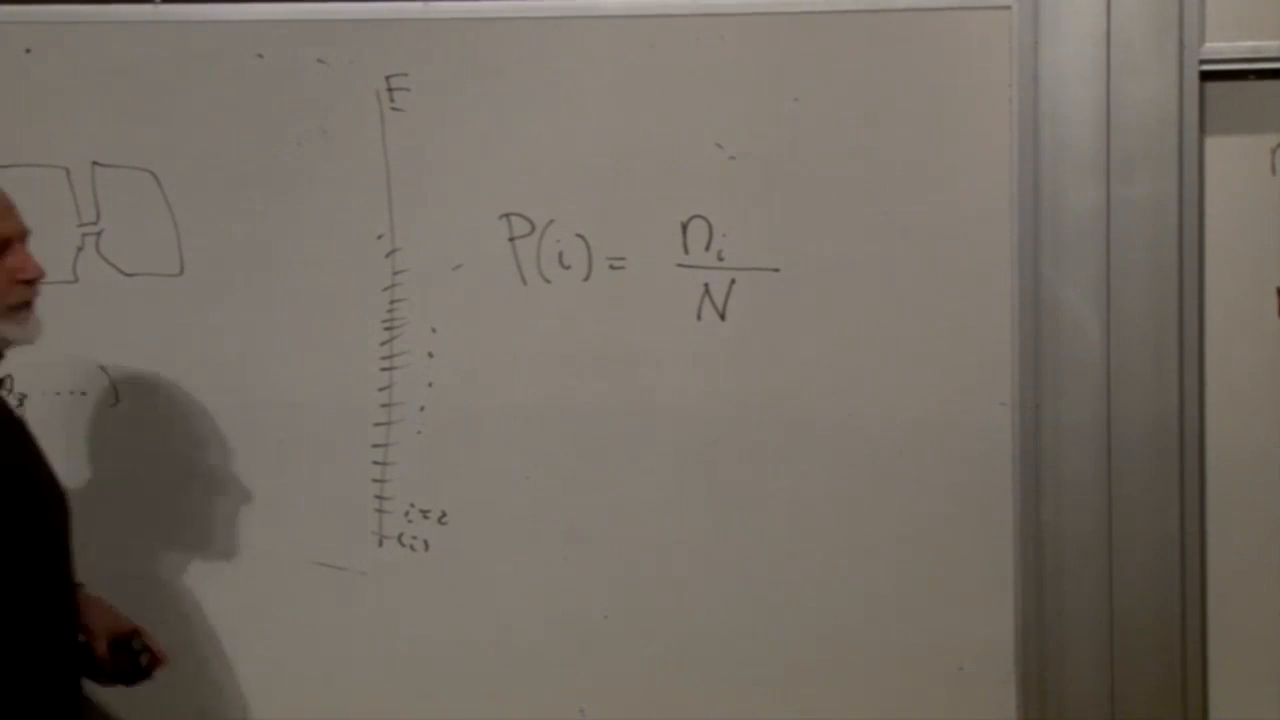
\includegraphics[width=0.82\textwidth]{lecture_03_figure_03.png}\caption{能階圖，以及將機率視為佔據比例\(P_i=n_i/N\)。}\lectureframe{00:41:40}\end{figure}

\begin{classroomqa}\audiencequestion{黑板上的記號\(N(i)\)是否有別於\(n_i\)？}\lecturerresponse{沒有。兩者都表示態\(i\)的佔據數。我們統一使用\(n_i\)，並以大寫\(N\)表示複本總數。\lecturetimestamp{00:41:28--00:41:33}}\end{classroomqa}

將\eqref{eq:sm3-number-constraint}與\eqref{eq:sm3-total-energy-constraint}除以\(N\)，便可還原為機率約束：\begin{equation}
 \sum_iP_i=1,
 \qquad
 \sum_iP_iE_i=\overline E.
 \label{eq:sm3-probability-constraints}
\end{equation}因此，以系綜頻率解釋機率，便重新得到一開始列出的方程式。

\section{佔據模式的多重度}

固定一組佔據數\(\{n_i\}\)。將\(N\)個可區分的複本分配到各個態，有多少種分配方式能恰好實現這組佔據數？答案是多項式係數：\begin{equation}
 C(\{n_i\})=\frac{N!}{\prod_i n_i!}.
 \label{eq:sm3-multiplicity}
\end{equation}來看分母的由來：先將全部\(N\)個帶有標記的複本排成\(N!\)種次序。處於同一態的\(n_i\)個複本彼此交換，不會形成新的佔據分配，因此每個態都要除以\(n_i!\)。

\begin{figure}[t]\centering
\includegraphics[width=0.88\textwidth]{lecture_03_figure_04.png}\caption{黑板上寫出的多項式多重度\(C=N!/\prod_i n_i!\)。}\lectureframe{00:46:55}\end{figure}

未佔據的能階不會造成問題，因為\(0!=1\)。若所有複本都處於同一態，則\[
 C=\frac{N!}{N!}=1,
\]結果如預期。若三個複本分別處於三個指定的不同態，則\[
 C=\frac{3!}{1!\,1!\,1!}=6.
\]若兩個複本分別處於兩個指定的態，公式給出兩種分配方式：交換兩個帶標記的複本所處的態。

\begin{classroomqa}\audiencequestion{是否可能有多組佔據數都滿足這兩項約束？}\lecturerresponse{通常有很多組。方程式\eqref{eq:sm3-multiplicity}先計算某一組固定佔據數\(\{n_i\}\)所對應的排列數，尚未判斷這組佔據數是否符合約束。下一步才是比較所有符合約束的組合，找出多重度最大的那一組。\lecturetimestamp{00:48:07--00:48:43}}\end{classroomqa}

統計假設是：對孤立系統而言，所有相容的微觀分配一視同仁。因此，能由較多分配方式實現的宏觀佔據模式，出現的機率也較高。當\(N\)很大時，分數\(n_i/N\)的分布會高度集中。平衡分數就是在滿足\eqref{eq:sm3-number-constraint}與\eqref{eq:sm3-total-energy-constraint}的條件下，使\(C\)最大的那些值。

\section{斯特林近似}

在\(N\)達到宏觀尺度之前，階乘就已經大得驚人，因此我們改用階乘的對數。先從\begin{equation}
 \log N!=\sum_{x=1}^{N}\log x.
 \label{eq:sm3-log-factorial-sum}
\end{equation}開始。當\(N\)很大時，這個總和可用\(\log x\)曲線下的面積近似：\begin{align}
 \log N!
 &\simeq\int_1^N\log x\,dx\\
 &=\left[x\log x-x\right]_1^N\\
 &=N\log N-N+1.
 \label{eq:sm3-stirling-integral}
\end{align}原函數可由\[
 \frac{d}{dx}(x\log x-x)=\log x.
\]直接得到。在領先的廣延階下，加法常數可以略去：\begin{equation}
 \log N!\simeq N\log N-N.
 \label{eq:sm3-stirling-log}
\end{equation}取指數後，得到講座中使用的簡化形式：\begin{equation}
 N!\simeq N^N e^{-N}.
 \label{eq:sm3-stirling-simple}
\end{equation}

\begin{figure}[t]\centering
\includegraphics[width=0.88\textwidth]{lecture_03_figure_05.png}\caption{將\(\log x\)的總和以積分近似，並由此推導領先階的斯特林近似。}\lectureframe{01:03:45}\end{figure}

\begin{classroomqa}\audiencequestion{在下限處計算\(x\log x-x\)，是否會多出一個\(+1\)？}\lecturerresponse{會。方程式\eqref{eq:sm3-stirling-integral}確實包含這個常數。當\(N\to\infty\)時，與正比於\(N\)的項相比，這個常數可以忽略，因此領先階公式省略了它。總和必須從\(x=1\)開始；\(\log0\)並無定義。\lecturetimestamp{01:04:12--01:04:35}}\end{classroomqa}

\begin{classroomqa}\audiencequestion{是否也漏掉了一個正比於\(\sqrt{N}\)的因子？}\lecturerresponse{是。較精確的漸近公式是\[
 N!\sim\sqrt{2\pi N}\left(\frac{N}{e}\right)^N.
\]其對數只會增加\(\tfrac12\log(2\pi N)\)，相較於\(N\log N-N\)，這是次廣延項。對精確計算有限\(N\)時的機率而言，它很重要；但對宏觀系統的領先階熵計算則無關緊要。\lecturetimestamp{01:04:35--01:05:40}}\end{classroomqa}

在\eqref{eq:sm3-multiplicity}的分母中使用斯特林近似時，也必須小心。在熱力學極限下，極限機率非零的狀態滿足\(n_i=NP_i\)，因此這些狀態的佔據數會隨\(N\)增大。佔據數極小或趨近於零的狀態，可以先以有限能量截斷處理，再透過取極限納入。省略次領先項不會影響領先階的廣延熵。

\section{多重度的對數就是熵}

將\eqref{eq:sm3-stirling-simple}用於分子以及所有宏觀佔據數很大的分母因子：\begin{equation}
 C\simeq
 \frac{N^Ne^{-N}}
 {\prod_i n_i^{\,n_i}e^{-n_i}}.
 \label{eq:sm3-c-stirling}
\end{equation}由於\(\sum_i n_i=N\)，領先階的指數因子會相消：\begin{equation}
 C\simeq\frac{N^N}{\prod_i n_i^{\,n_i}}.
 \label{eq:sm3-c-leading}
\end{equation}對數函數是單調的，因此最大化對數比最大化乘積容易，而且兩者的最大值出現在同一組佔據數上：\begin{equation}
 \log C=N\log N-\sum_i n_i\log n_i.
 \label{eq:sm3-logc-occupations}
\end{equation}現在代入\(n_i=NP_i\)：\begin{align}
 \log C
 &=N\log N-\sum_iNP_i\log(NP_i)\\
 &=N\log N-N\sum_iP_i\log N
   -N\sum_iP_i\log P_i\\
 &=-N\sum_iP_i\log P_i,
 \label{eq:sm3-logc-entropy-derivation}
\end{align}其中，歸一化條件使兩個\(N\log N\)項相消。因此，在\(N\)的領先階下，\begin{equation}
 \boxed{\log C=NS}.
 \label{eq:sm3-logc-ns}
\end{equation}

\begin{figure}[t]\centering
\includegraphics[width=0.88\textwidth]{lecture_03_figure_06.png}\caption{黑板上的推導將\(\log C=N\log N-\sum_i n_i\log n_i\)與\(-N\sum_iP_i\log P_i=NS\)連結起來。}\lectureframe{01:16:10}\end{figure}

這個關係是本章的核心概念。熵不是另外加到計數問題上的無關量，而是以對數表示、按複本計算的多重度。因此，在領先階下，最大化微觀排列數，就等同於最大化單一複本的熵。

\begin{classroomqa}\audiencequestion{若所有佔據數都相等，多重度不是應該最大嗎？}\lecturerresponse{若沒有特別區分任何狀態，且唯一的約束是在有限狀態集合上滿足\(\sum_i n_i=N\)，分布便是均勻的。但固定能量的約束會改變答案，因為各個\(E_i\)的值並不相同。一般而言，佔據數相等無法符合指定的平均能量。\lecturetimestamp{01:17:07--01:18:20}}\end{classroomqa}

\begin{classroomqa}\audiencequestion{大寫\(N\)很大，但為什麼可以對分母中的每個\(n_i\)都使用斯特林近似？}\lecturerresponse{對每個極限機率非零的狀態，\(n_i=NP_i\)都會隨\(N\)成比例增大。可以先只保留有限的能量範圍，在此範圍內取\(N\)趨近無限大的極限，再逐步擴大能量範圍。佔據稀疏的尾端狀態需要另行計入有限修正，但不會改變領先階的廣延熵。\lecturetimestamp{01:18:23--01:19:28}}\end{classroomqa}

\begin{classroomqa}\audiencequestion{這裡所說的大\(N\)近似，就是前面提到的粗粒化嗎？}\lecturerresponse{不是。熱力學極限處理的是大佔據數與漸近計數；粗粒化則是微觀解析度的流失或刻意捨棄。兩者是不同的操作，雖然在宏觀統計力學中常會同時用到。\lecturetimestamp{01:19:29--01:19:46}}\end{classroomqa}

\begin{classroomqa}\audiencequestion{既然\(\log C=N\log N-\sum_i n_i\log n_i\)，第二項不是應該最小化，而非最大化嗎？}\lecturerresponse{是；在\(N\)固定時，最大化\(\log C\)等同於最小化\(\sum_i n_i\log n_i\)。代入\(n_i=NP_i\)後，固定的\(N\log N\)項會相消，剩下\(-N\sum_iP_i\log P_i=NS\)。因此，更自然的說法是最大化正值的熵\(S\)。\lecturetimestamp{01:19:48--01:20:55}}\end{classroomqa}

\begin{classroomqa}\audiencequestion{為什麼不直接利用對稱性，令所有\(n_i\)相等，立即完成論證？}\lecturerresponse{這種捷徑忽略了能量標記。歸一化約束對各個狀態一視同仁，但\(\sum_iP_iE_i=\overline E\)並非如此：能量不同的狀態，其貢獻也不同。非均勻的平衡分布正是由能量約束所決定。\lecturetimestamp{01:21:15--01:21:41}}\end{classroomqa}

\section{最大熵問題}

現在可以明確陳述統計力學的規則：改變機率\(P_i\)，使\begin{equation}
 S[P]=-\sum_iP_i\log P_i
 \label{eq:sm3-maximize-entropy}
\end{equation}最大，並滿足下列條件：\begin{equation}
 \sum_iP_i=1,
 \qquad
 \sum_iP_iE_i=\overline E.
 \label{eq:sm3-maxent-constraints}
\end{equation}最大化所得的機率，給出大型複本系綜中最受偏好的佔據比例。佔據數仍會漲落，但隨著\(N\)增大，其相對偏差會縮小，因此比值\(n_i/N\)會成為定義良好的熱力學機率。

\begin{classroomqa}\audiencequestion{\(E_i\)是固定的態能量，而約束條件使用的是另行給定的總能量嗎？}\lecturerresponse{是。能譜\(\{E_i\}\)屬於子系統。整個複本集合的總能量固定，但能量會持續在複本之間轉移。總能量除以\(N\)所得到的是單一複本的平均能量\(\overline E\)，並非每次微觀實現中的能量。\lecturetimestamp{01:26:12--01:27:07}}\end{classroomqa}

這個問題很容易表述，但還沒有解出。這是帶有兩項約束的極值問題，因此還需要一種數學工具。

\section{拉格朗日乘數}

對於無約束函數\(F(x_1,x_2,\ldots)\)，駐點須滿足\begin{equation}
 \frac{\partial F}{\partial x_i}=0
 \qquad\text{for every }i.
 \label{eq:sm3-unconstrained-stationary}
\end{equation}現在再加上條件\begin{equation}
 G(x_1,x_2,\ldots)=0.
 \label{eq:sm3-one-constraint}
\end{equation}

\begin{classroomqa}\audiencequestion{如果圖中的座標是\(x\)與\(y\)，那麼\(x\)代表什麼？}\lecturerresponse{這裡的\(x\)是整個座標向量\((x_1,x_2,\ldots)\)的簡寫。在二維圖中，其分量就是\(x\)與\(y\)。之後，各分量會是機率\(P_1,P_2,\ldots\)。\lecturetimestamp{01:30:12--01:30:20}}\end{classroomqa}

從幾何上看，等值線\(F=\text{constant}\)構成一幅等高線圖，而\(G=0\)則是系統可沿之移動的曲線。當\(F\)的一條等值線與約束曲線相切時，就會出現約束極值。在切點處，兩個梯度彼此平行：\begin{equation}
 \nabla F=-\lambda\nabla G
 \label{eq:sm3-parallel-gradients}
\end{equation}其中\(\lambda\)為某個數值。

\begin{figure}[t]\centering
\includegraphics[width=0.88\textwidth]{lecture_03_figure_07.png}\caption{黑板上的等值線幾何與增廣函數\(F'=F+\lambda G\)。約束極值出現在相切處。}\lectureframe{01:37:10}\end{figure}

定義增廣函數\begin{equation}
 F'=F+\lambda G
 \label{eq:sm3-augmented-function}
\end{equation}，並要求其滿足一般的駐點條件\begin{equation}
 \frac{\partial F'}{\partial x_i}=0.
 \label{eq:sm3-augmented-stationarity}
\end{equation}，即可得到方程式\eqref{eq:sm3-parallel-gradients}。乘數\(\lambda\)起初未知，但這並不會使方程組欠定，因為原本的約束\(G=0\)會再提供一個方程式。

\begin{classroomqa}\classquestion{為什麼加上與\(G\)成正比的一項，就能使約束點成為駐點？}\lecturerresponse{在約束極值處，沿著\(G=0\)切線方向移動，已不會使\(F\)產生一階變化。剩下的斜率只有垂直於約束曲線的分量。由於\(\nabla G\)指向同一法線方向，適當選取\(\lambda\)便能抵銷這個分量：\(\nabla F+\lambda\nabla G=0\)。\lecturetimestamp{01:35:06--01:35:32}}\end{classroomqa}

\section{二變數範例}

求下式的最小值：\begin{equation}
 F(x,y)=\frac{x^2+y^2}{2}
 \label{eq:sm3-example-f}
\end{equation}約束條件為\begin{equation}
 x+y=1.
 \label{eq:sm3-example-constraint}
\end{equation}將約束寫成\(G=x+y-1=0\)，並構造增廣函數\begin{equation}
 F'=\frac{x^2+y^2}{2}+\lambda(x+y-1).
 \label{eq:sm3-example-augmented}
\end{equation}駐點方程式為\begin{align}
 \frac{\partial F'}{\partial x}&=x+\lambda=0,\\
 \frac{\partial F'}{\partial y}&=y+\lambda=0.
 \label{eq:sm3-example-derivatives}
\end{align}因此\(x=y=-\lambda\)。剩下的方程式就是約束條件：\[
 x+y=-2\lambda=1,
\]所以\begin{equation}
 \lambda=-\frac12,
 \qquad
 x=y=\frac12.
 \label{eq:sm3-example-solution}
\end{equation}點\((1/2,1/2)\)是以原點為圓心的最小圓與直線\(x+y=1\)的切點。

\begin{figure}[t]\centering
\includegraphics[width=0.88\textwidth]{lecture_03_figure_08.png}\caption{在約束\(x+y=1\)下，求\((x^2+y^2)/2\)最小值的拉格朗日乘數計算。}\lectureframe{01:44:10}\end{figure}

若有多項約束，就為每項約束引入一個乘數：\begin{equation}
 F'=F+\lambda_1G_1+\lambda_2G_2+\cdots.
 \label{eq:sm3-many-multipliers}
\end{equation}接著求解\begin{equation}
 \begin{aligned}
 \frac{\partial F'}{\partial x_i}&=0
 &&\text{for every }i,\\
 G_a&=0
 &&\text{for every constraint }a.
 \end{aligned}
 \label{eq:sm3-many-equations}
\end{equation}講座提出一道刻意設計得很不實際的練習題：對\(x,y,z\)的二次函數求極值，同時施加兩項獨立的線性約束，例如\(x+y=1\)與\(z+x=1\)。重點不在特定的答案，而在於掌握這項規則：每項約束都會帶來一個乘數與一個方程式。

\section{留待下一講求解的問題}

在統計力學中，座標是機率\(\{P_i\}\)，要最大化的函數是熵，而約束條件是歸一化與平均能量固定。定義\begin{align}
 S[P]&=-\sum_iP_i\log P_i,\\
 G_1[P]&=\sum_iP_i-1,\\
 G_2[P]&=\sum_iP_iE_i-\overline E.
 \label{eq:sm3-final-functions}
\end{align}因此，增廣熵可以寫成\begin{equation}
 \Phi[P]
 =S[P]+\alpha G_1[P]+\beta G_2[P].
 \label{eq:sm3-final-augmented}
\end{equation}待求解的方程式為\begin{equation}
 \frac{\partial\Phi}{\partial P_i}=0
 \quad\text{for every }i,
 \qquad
 G_1=0,
 \qquad
 G_2=0.
 \label{eq:sm3-final-problem}
\end{equation}

\begin{figure}[H]\centering
\includegraphics[width=0.88\textwidth]{lecture_03_figure_09.png}\caption{最後的板書：以機率為變數的熵，以及歸一化與平均能量固定這兩項條件。}\lectureframe{01:53:05}\end{figure}

至此，問題已完整設定。求解\eqref{eq:sm3-final-problem}即可得到平衡分布。與能量共軛的乘數將成為逆溫度\(\beta=1/T\)，其正負號取決於\eqref{eq:sm3-final-augmented}所採用的符號慣例。下一講將進行微分，推導出玻爾茲曼權重。